\chapter{Advanced simulations of the Ising model}

\section{Wolff cluster algorithm}

\begin{sourcefiles}
  \item[Source code] src/061\_ising\_wolff.c
  \item[Analysis script] src/061\_ising\_wolff.R
  \item[Executable] exe/061\_ising\_wolff
\end{sourcefiles}

For the first part of the exercise, I ran three simulations on a lattice of $N =
50 \times 50$ spins at three different temperatures: $T_{\mathrm{c}} / 2$,
$T_{\mathrm{c}}$ and $2 T_{\mathrm{c}}$, each lasting \num{500000} time steps.
The histograms of cluster sizes, shown in \cref{fig:061a,fig:061b,fig:061c},
exhibit expected profiles. The histogram at low temperature (\cref{fig:061a}),
is strongly bimodal with the largest peak around \num{2500} -- corresponding to
events where the entire lattice is flipped -- and a rather smaller peak around
\num{1}, representing the clusters that do not spread beyond the first few
spins. This is the expected behaviour in the ferromagnetic phase, since
$P_{\mathrm{add}}$ is high. In contrast, the histogram at high temperature
(\cref{fig:061c}) shows almost a power-law distribution, with smaller sized
clusters being predominant. The behaviour at the critical point
(\cref{fig:061b}) is intermediate between the ferromagnetic and paramagnetic
histograms: the distribution is still bimodal, but cluster sizes near \num{1}
are the most frequent, and the peak at larger sizes is wider and shifted to the
left. Indeed, at the critical point we expect large \enquote{seas} of correlated
spins, though not encompassing the whole lattice.

\begin{figure}
  \centering
  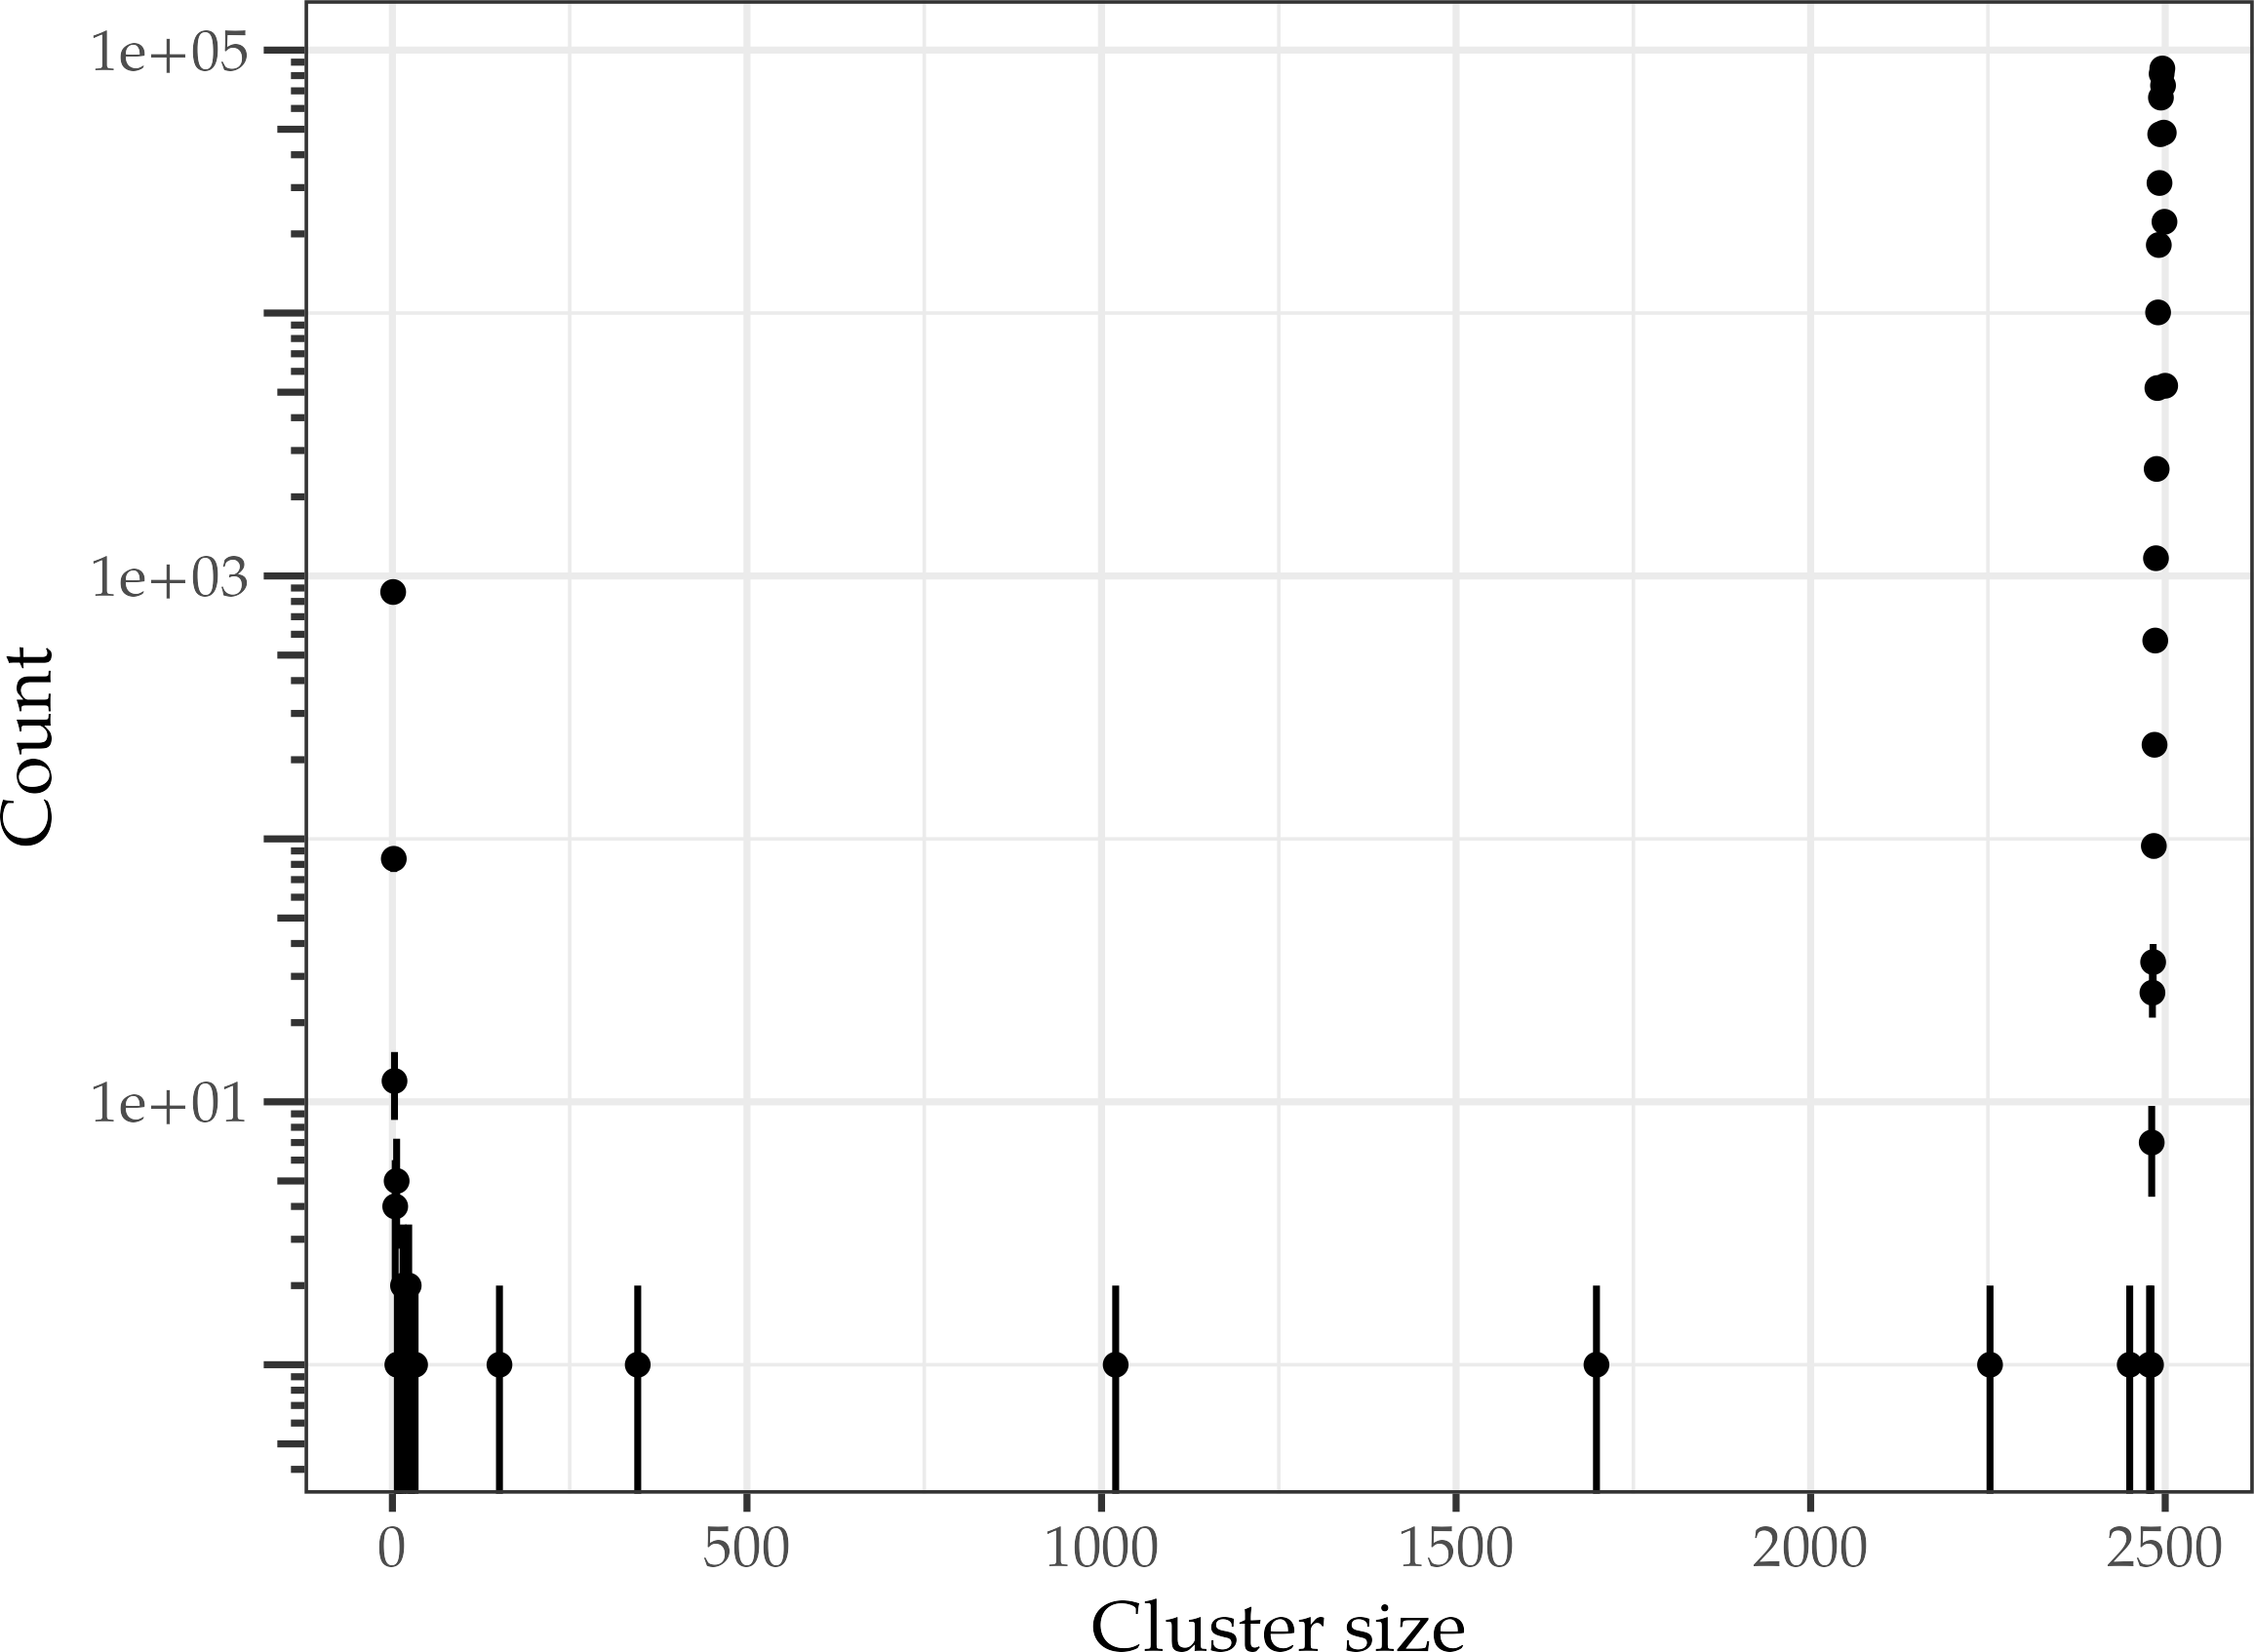
\includegraphics{img/061a.png}
  \caption{histogram of cluster sizes obtained from a Wolff algorithm simulation
    with $N = \num{2500}$ spins, run at a temperature $T = T_{\mathrm{c}} / 2$
    over \num{500000} time steps. Error bars represent Poissonian
    uncertainties.}
  \label{fig:061a}
\end{figure}

\begin{figure}
  \centering
  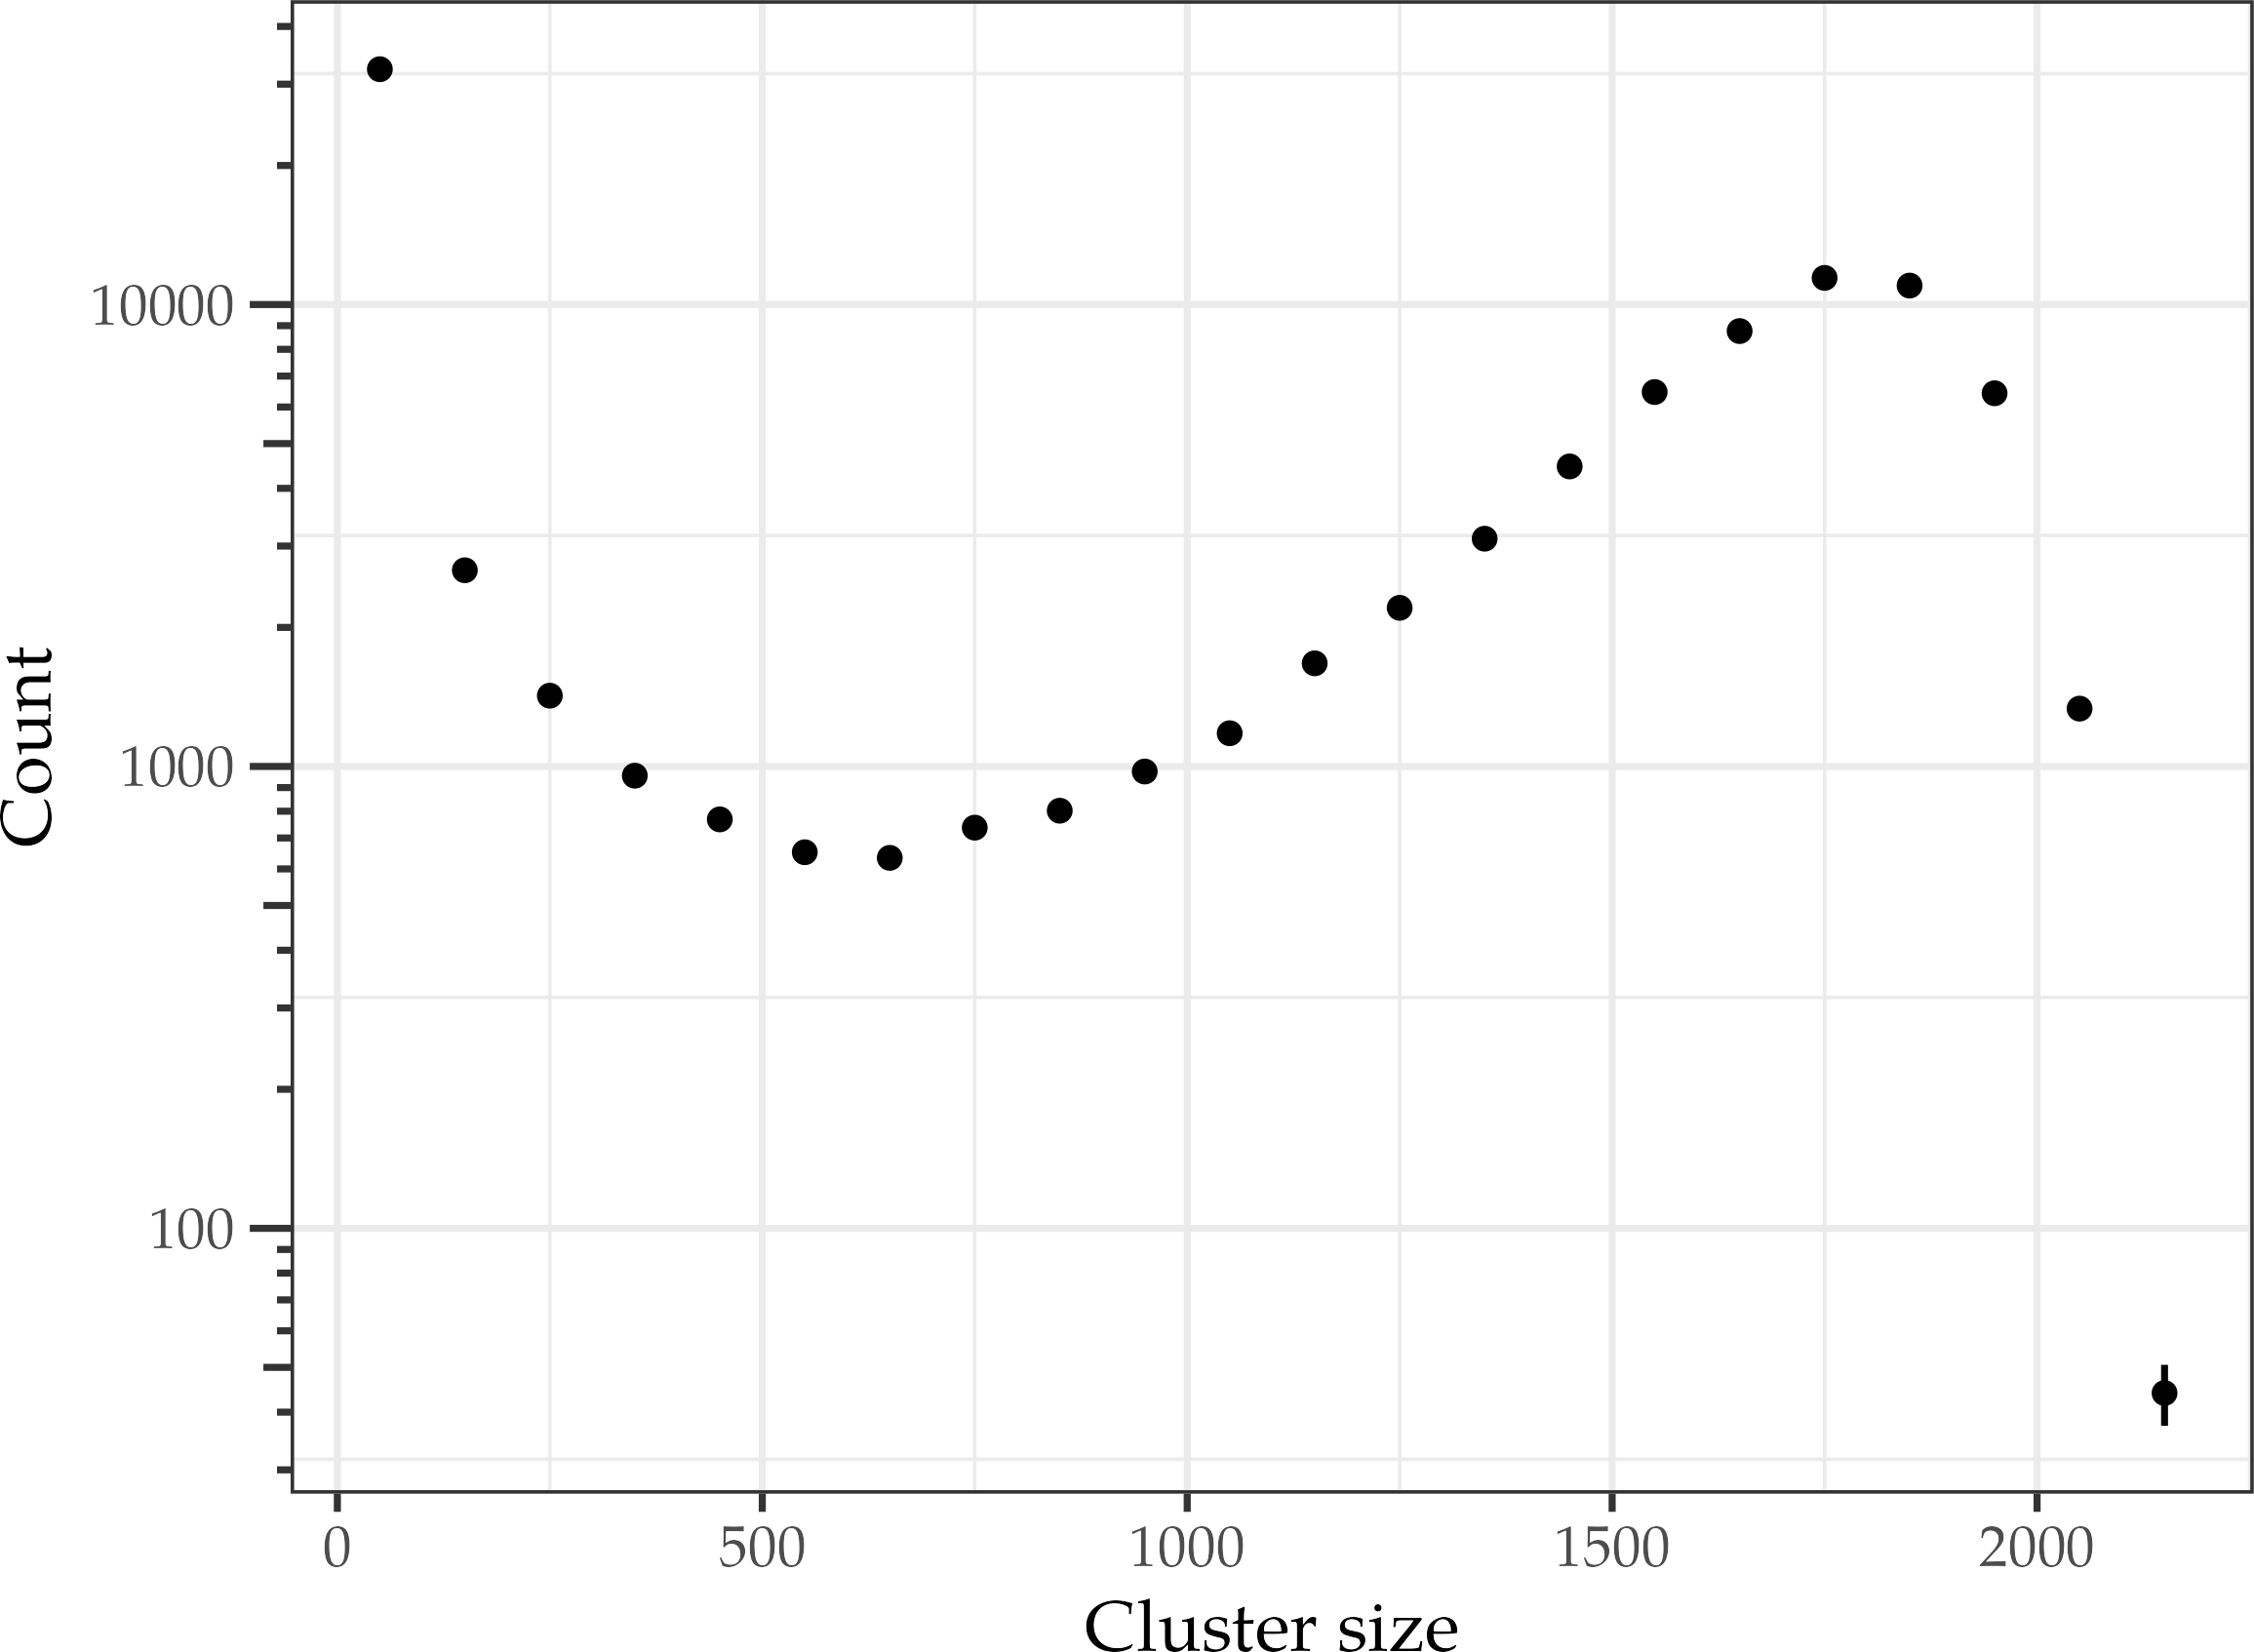
\includegraphics{img/061b.png}
  \caption{histogram of cluster sizes obtained from a Wolff algorithm simulation
    with $N = \num{2500}$ spins, run at a temperature $T = T_{\mathrm{c}}$
    over \num{500000} time steps. Error bars represent Poissonian
    uncertainties.}
  \label{fig:061b}
\end{figure}

\begin{figure}
  \centering
  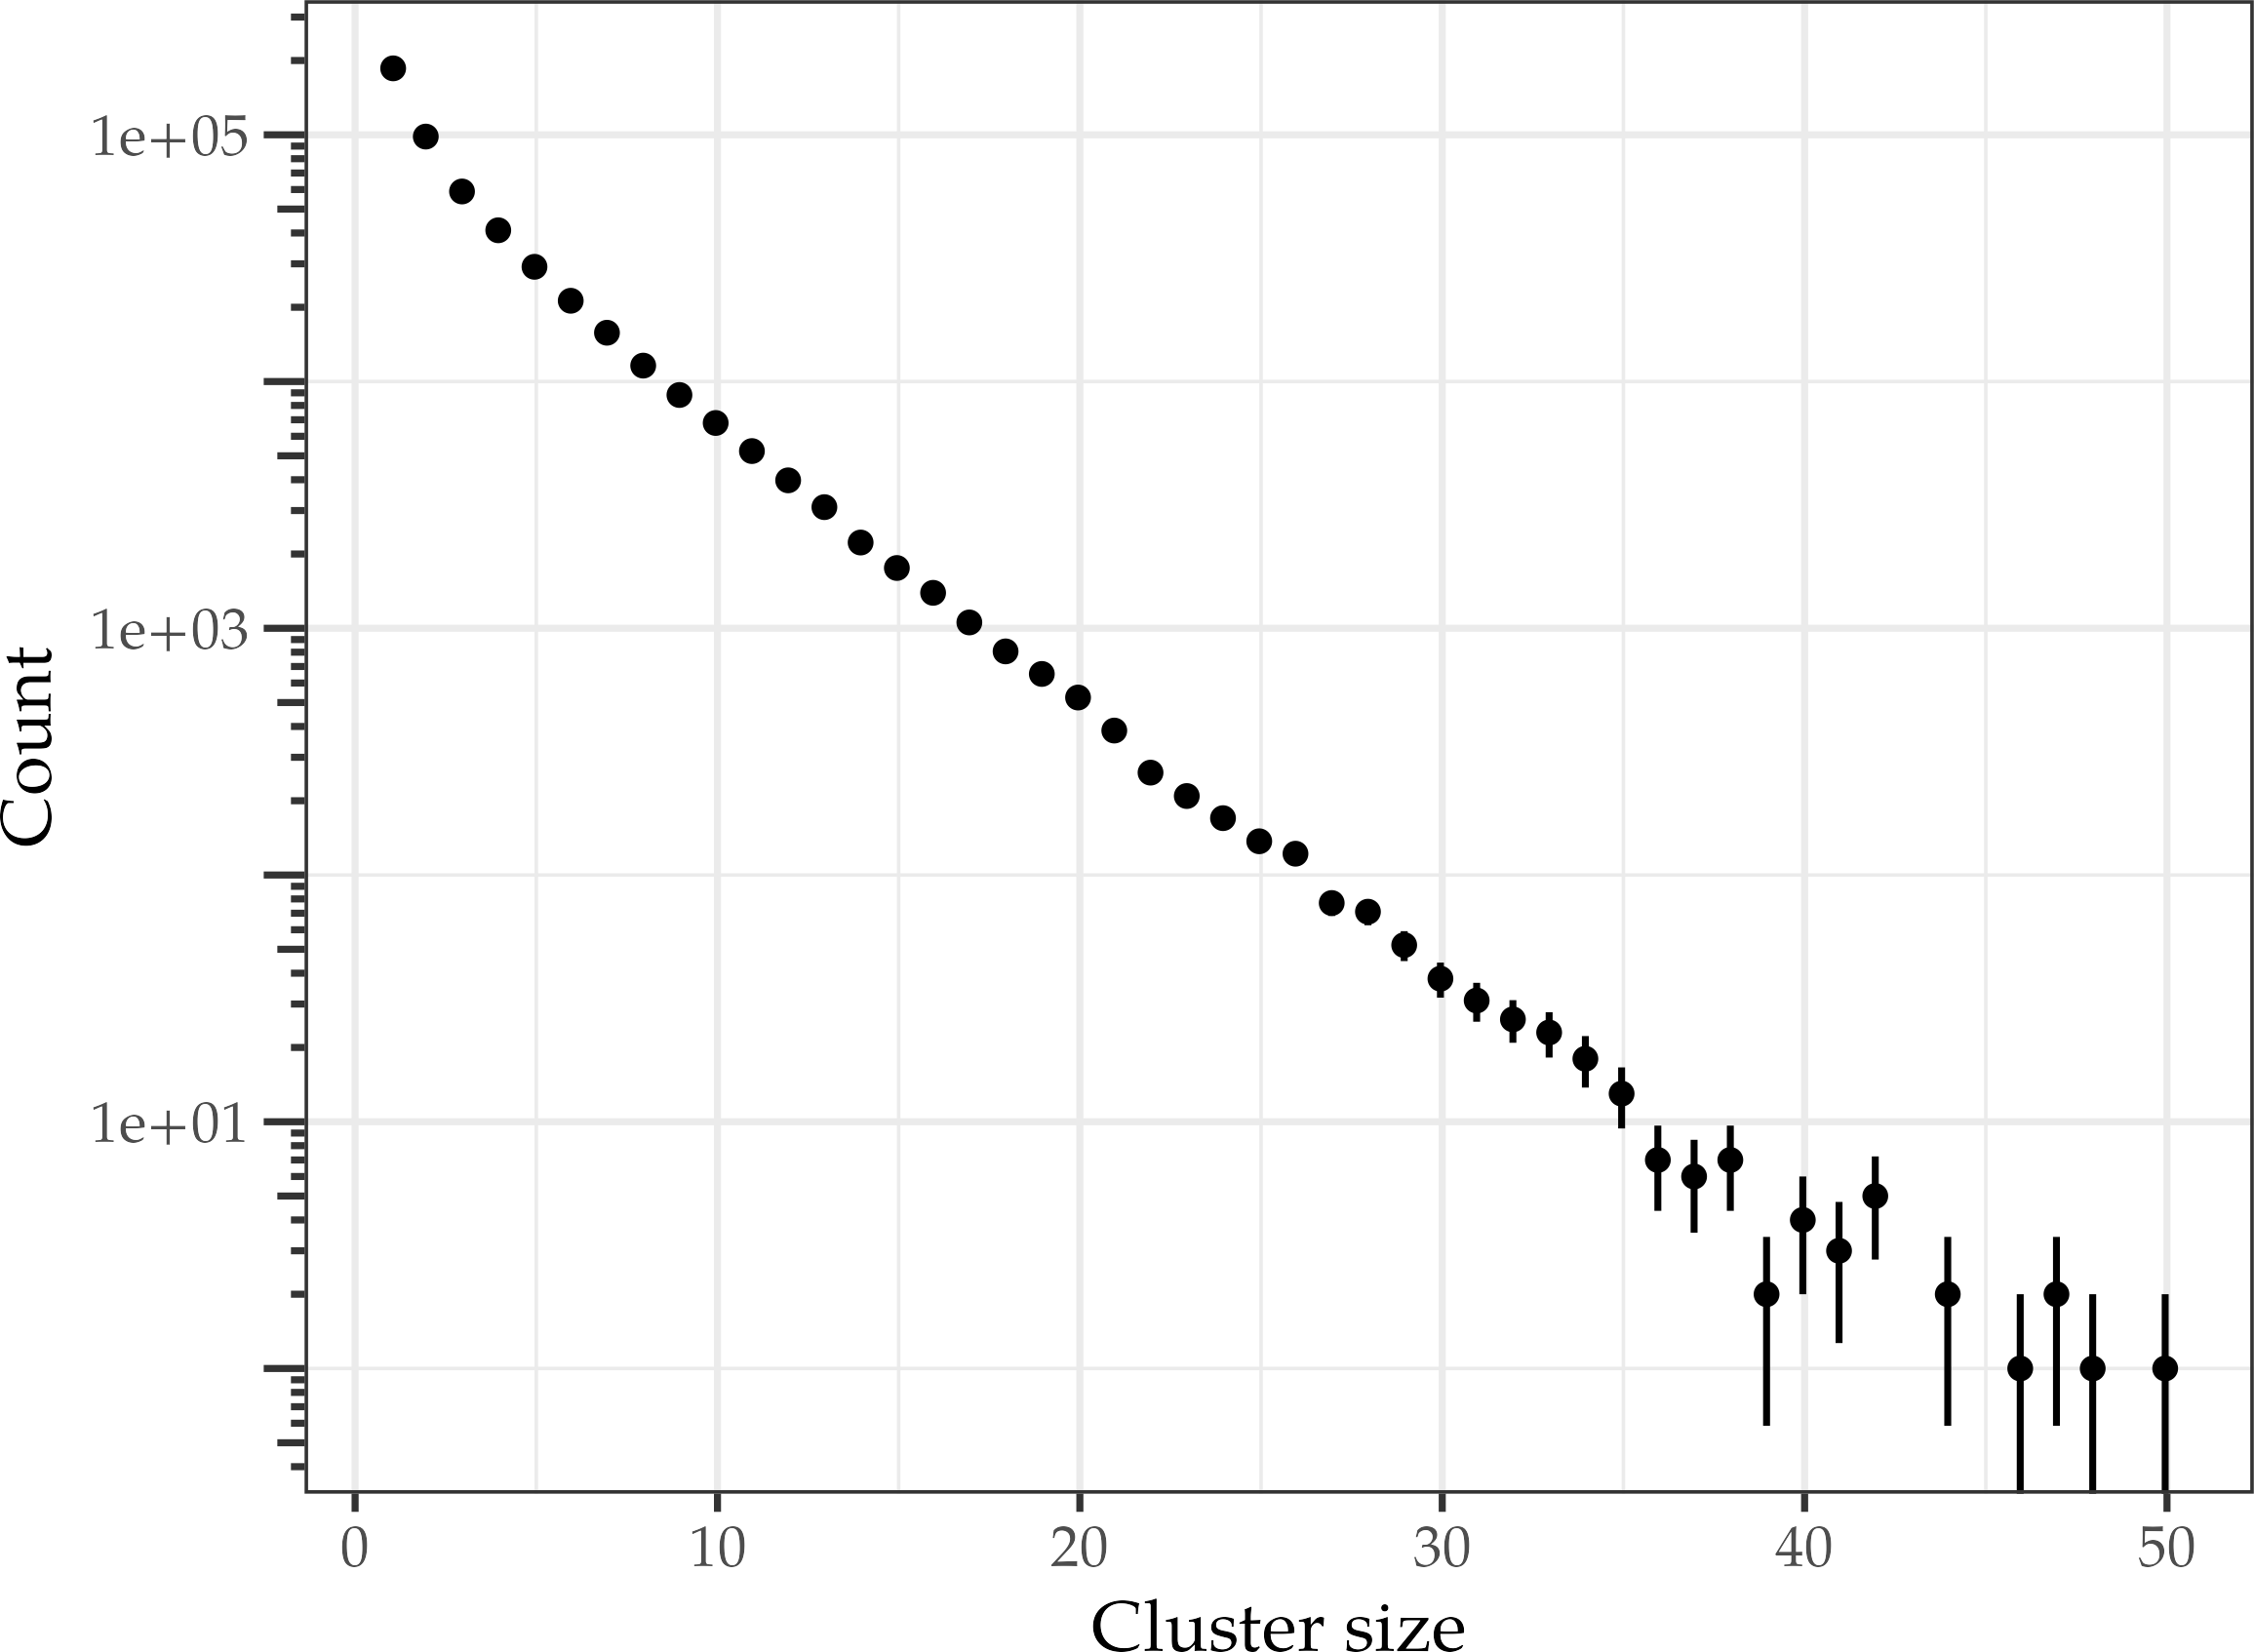
\includegraphics{img/061c.png}
  \caption{histogram of cluster sizes obtained from a Wolff algorithm simulation
    with $N = \num{2500}$ spins, run at a temperature $T = 2 T_{\mathrm{c}}$
    over \num{500000} time steps. Error bars represent Poissonian
    uncertainties.}
  \label{fig:061c}
\end{figure}

In the second part of the exercise, I examined the relationship between the
autocorrelation time of the observed energy and magnetization with the lattice
size, $L$, for both the Metropolis single spin-flip algorithm and the Wolff
algorithm. The aim was to validate the scaling relation $\tau \sim L^{z}$, with
the expectation that $z$ would be smaller in the case of the Wolff algorithm. I
conducted two sets of simulations, running each algorithm with $L \in \{10, 14,
20, 28, 40, 50\}$ at the critical temperature $T_{\mathrm{c}}$ for \num{1000000}
time steps. From each dataset, I computed the autocorrelation time of the energy
and magnetization time series, after discounting the equilibration phase. For
the Wolff algorithm, I adjusted $\tau$ by multiplying it by a factor of
$\mathcal{S} / L^{2}$, with $\mathcal{S}$ being the average cluster size at the
given temperature and lattice size.

\begin{figure}
  \centering
  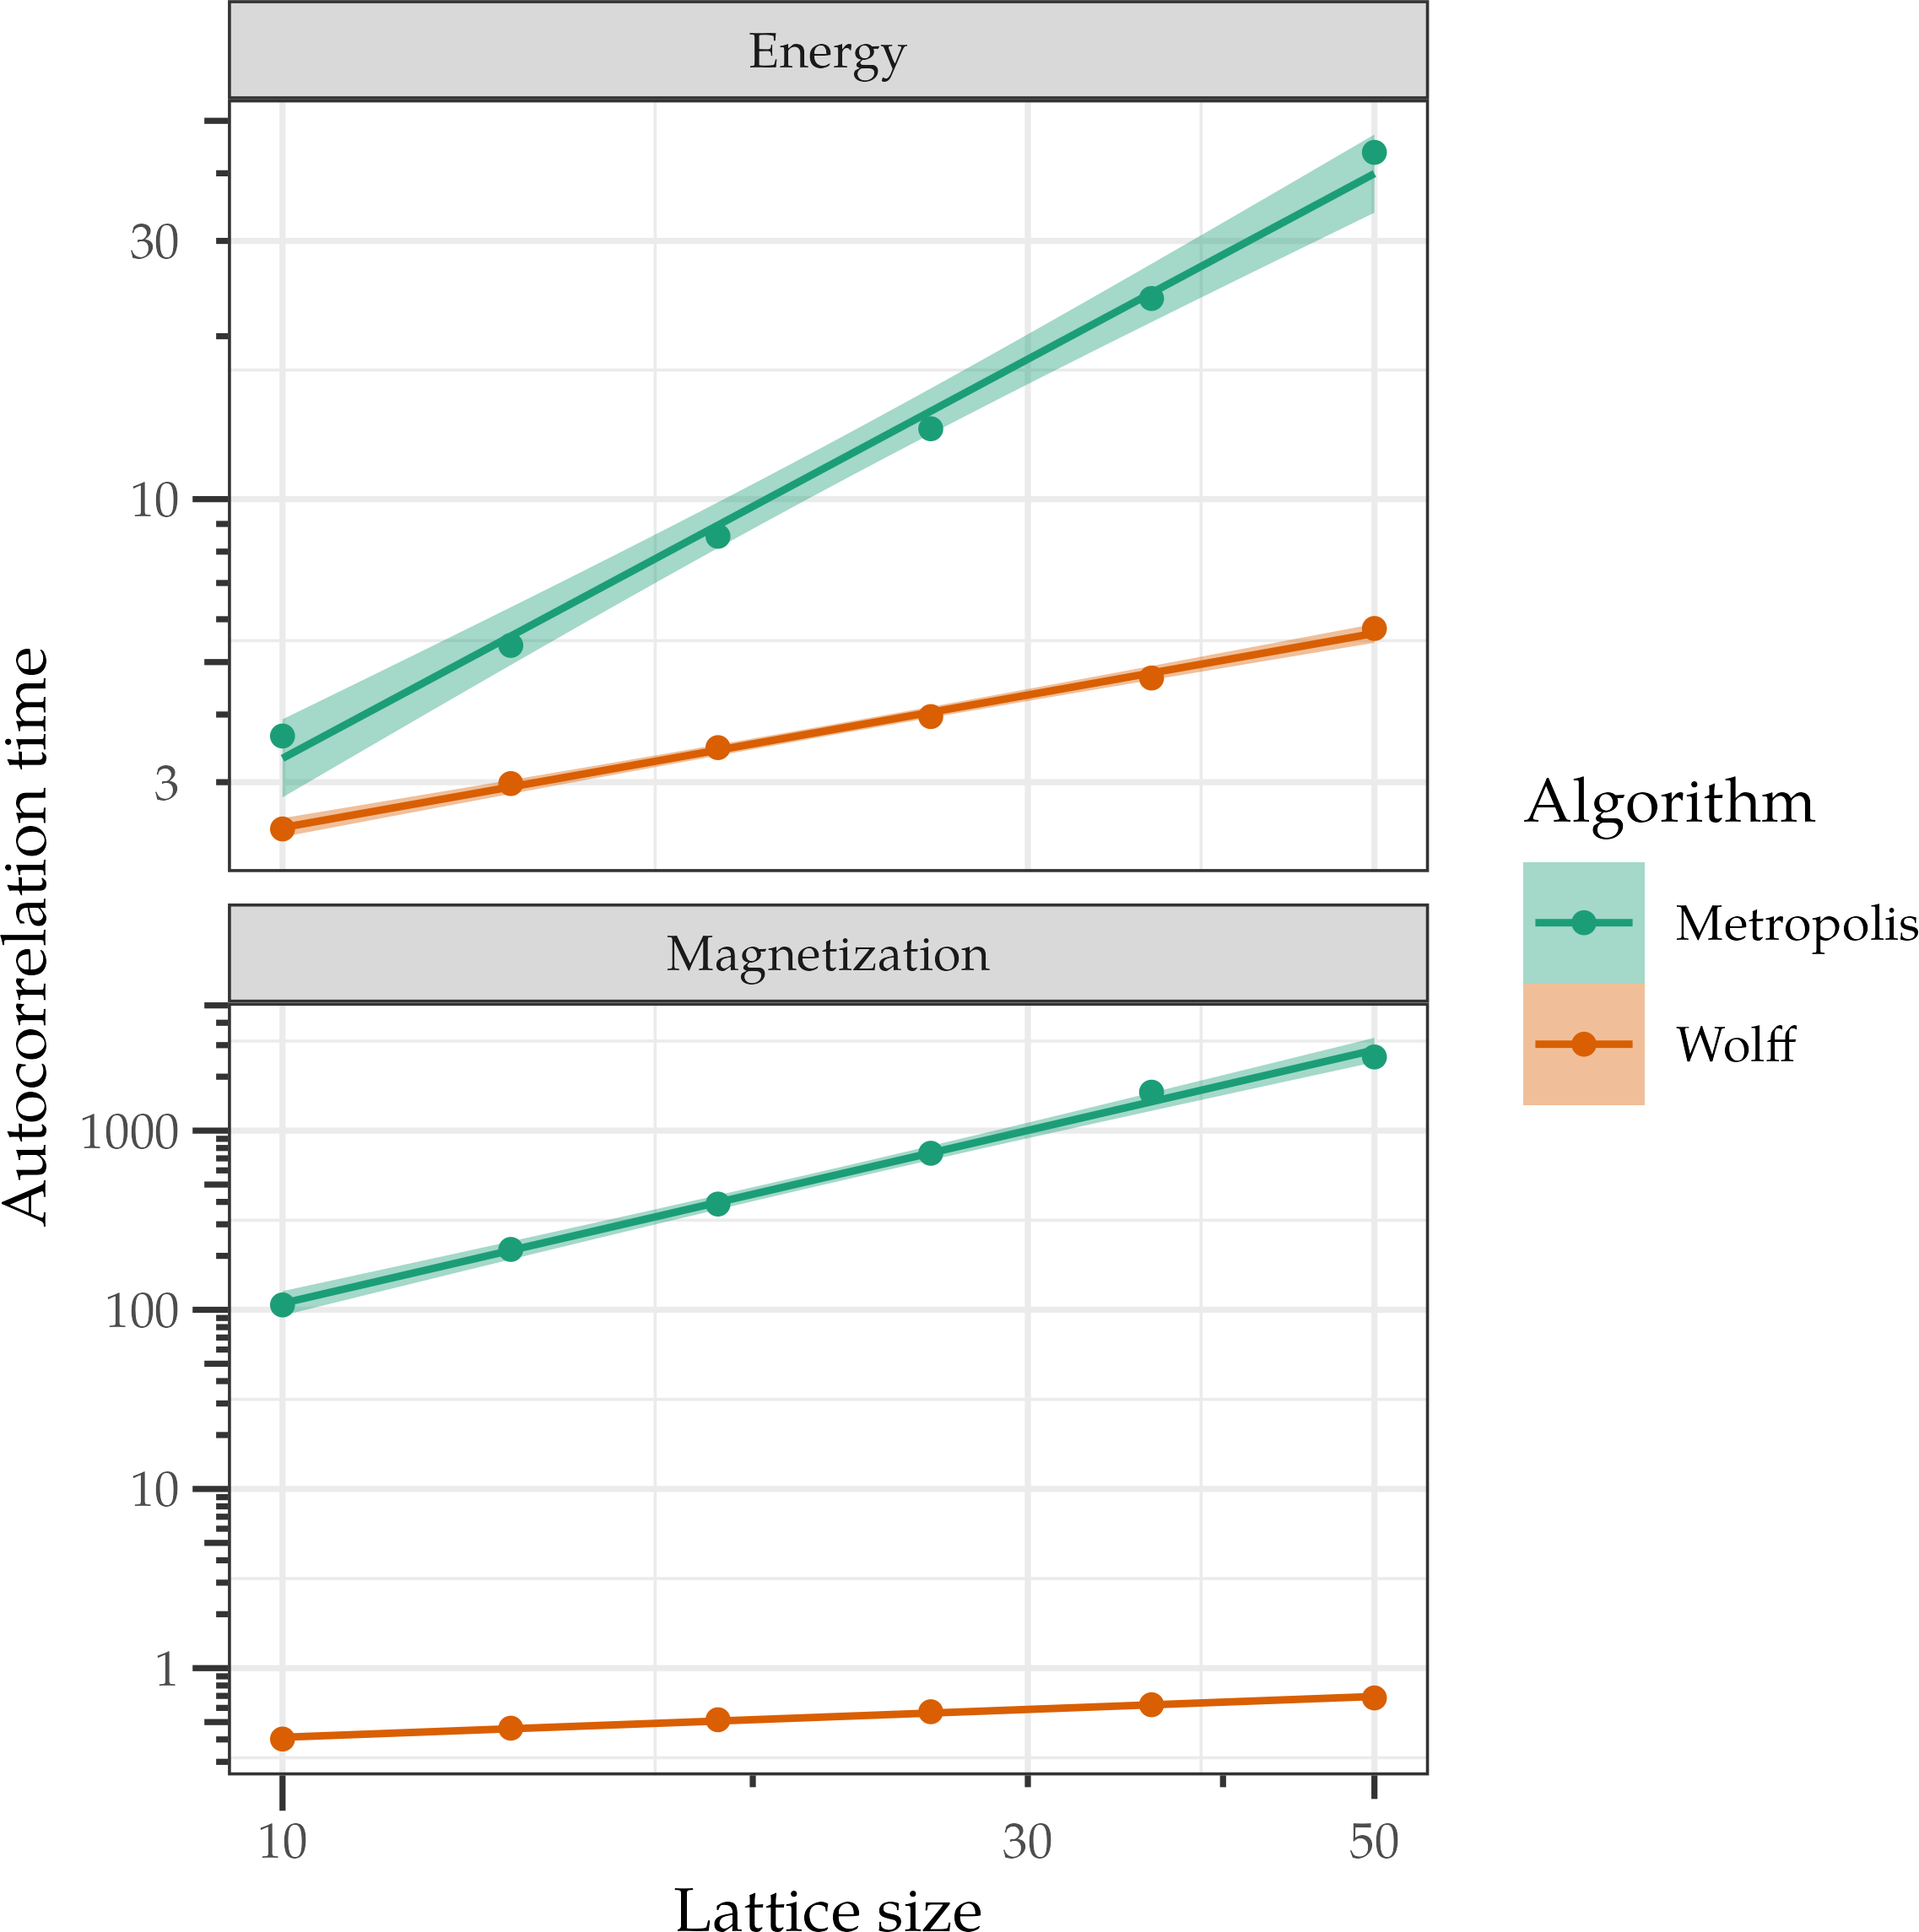
\includegraphics{img/061d.png}
  \caption{autocorrelation time of energy and magnetization as a function of the
    lattice size for the Metropolis and Wolff algorithms. Each run lasted
    \num{1000000} time steps. The parameters of the fitted lines are reported in
    \cref{tab:061}.}
  \label{fig:061d}
\end{figure}

\begin{table}
  \centering
  \captionabove{parameters of the $\log \tau \sim \log L$ linear fits from
    \cref{fig:061d}.}
  \label{tab:061}
  \begin{tabular}{
    @{}
    l l l
    S[table-format=+1.2(1)] S[table-format=+2.1] S[table-format=1.1e-1]
    @{}
  }
    \toprule
    Algorithm & Observable & Parameter & {Estimate} & {\textit{t}-statistic} &
    {\textit{p}-value} \\
    \midrule
    Metropolis & Energy & Intercept & -0.9(2) & -5.5 & 5.2e-3 \\
    Metropolis & Energy & Slope & 1.16(4) & 27 & 1.1e-5 \\
    Metropolis & Magnetization & Intercept & -0.5(2) & -2.2 & 8.9e-2 \\
    Metropolis & Magnetization & Slope & 1.30(6) & 21 & 2.9e-5 \\
    Wolff & Energy & Intercept & -0.70(9) & -7.8 & 1.5e-3 \\
    Wolff & Energy & Slope & 0.34(2) & 15 & 1.2e-4 \\
    Wolff & Magnetization & Intercept & -0.6(1) & -4.0 & 1.6e-2 \\
    Wolff & Magnetization & Slope & 0.21(3) & 6.0 & 3.8e-3 \\
    \bottomrule
  \end{tabular}
\end{table}

A log-log plot of $\tau$ as a function of $L$, separated by algorithm and
observable, is presented in \cref{fig:061d}. The parameters of the fitted lines
are listed in \cref{tab:061}. The slope ($z$) for Wolff's magnetization is in
sufficient agreement with the expected value of $z \approx 0.25$, while the
energy $z$ comes out slightly larger. Another result in line with expectations
is the smaller exponent $z$ for the Wolff algorithm, observed for both energy
and magnetization. In general, all autocorrelation times for the Metropolis
algorithm are larger than those for the Wolff algorithm, particularly at larger
lattice sizes. This is consistent with the expectation that the Wolff algorithm
is significantly more efficient than the Metropolis algorithm near
$T_{\mathrm{c}}$.

\section{Multiple Markov chains}

\begin{sourcefiles}
  \item[Source code] src/062\_ising\_mmc.c
  \item[Analysis script] src/062\_ising\_mmc.R
  \item[Executable] exe/062\_ising\_mmc
\end{sourcefiles}

In \texttt{src/062\_ising\_mmc.c}, I introduced the \enquote{multiple Markov
chains} schema over an underlying Metropolis algorithm implementation. The
program sets up $M$ identical Ising lattices, along with an array of
temperatures and another array linking each temperature to its associated
system. The lattices evolve independently until, after a certain number of time
steps, a \enquote{swap trial} occurs. If the swap is accepted based on the
Metropolis criterion, I simply swap the two pointers linking the temperatures to
the systems. 

\begin{figure}
  \centering
  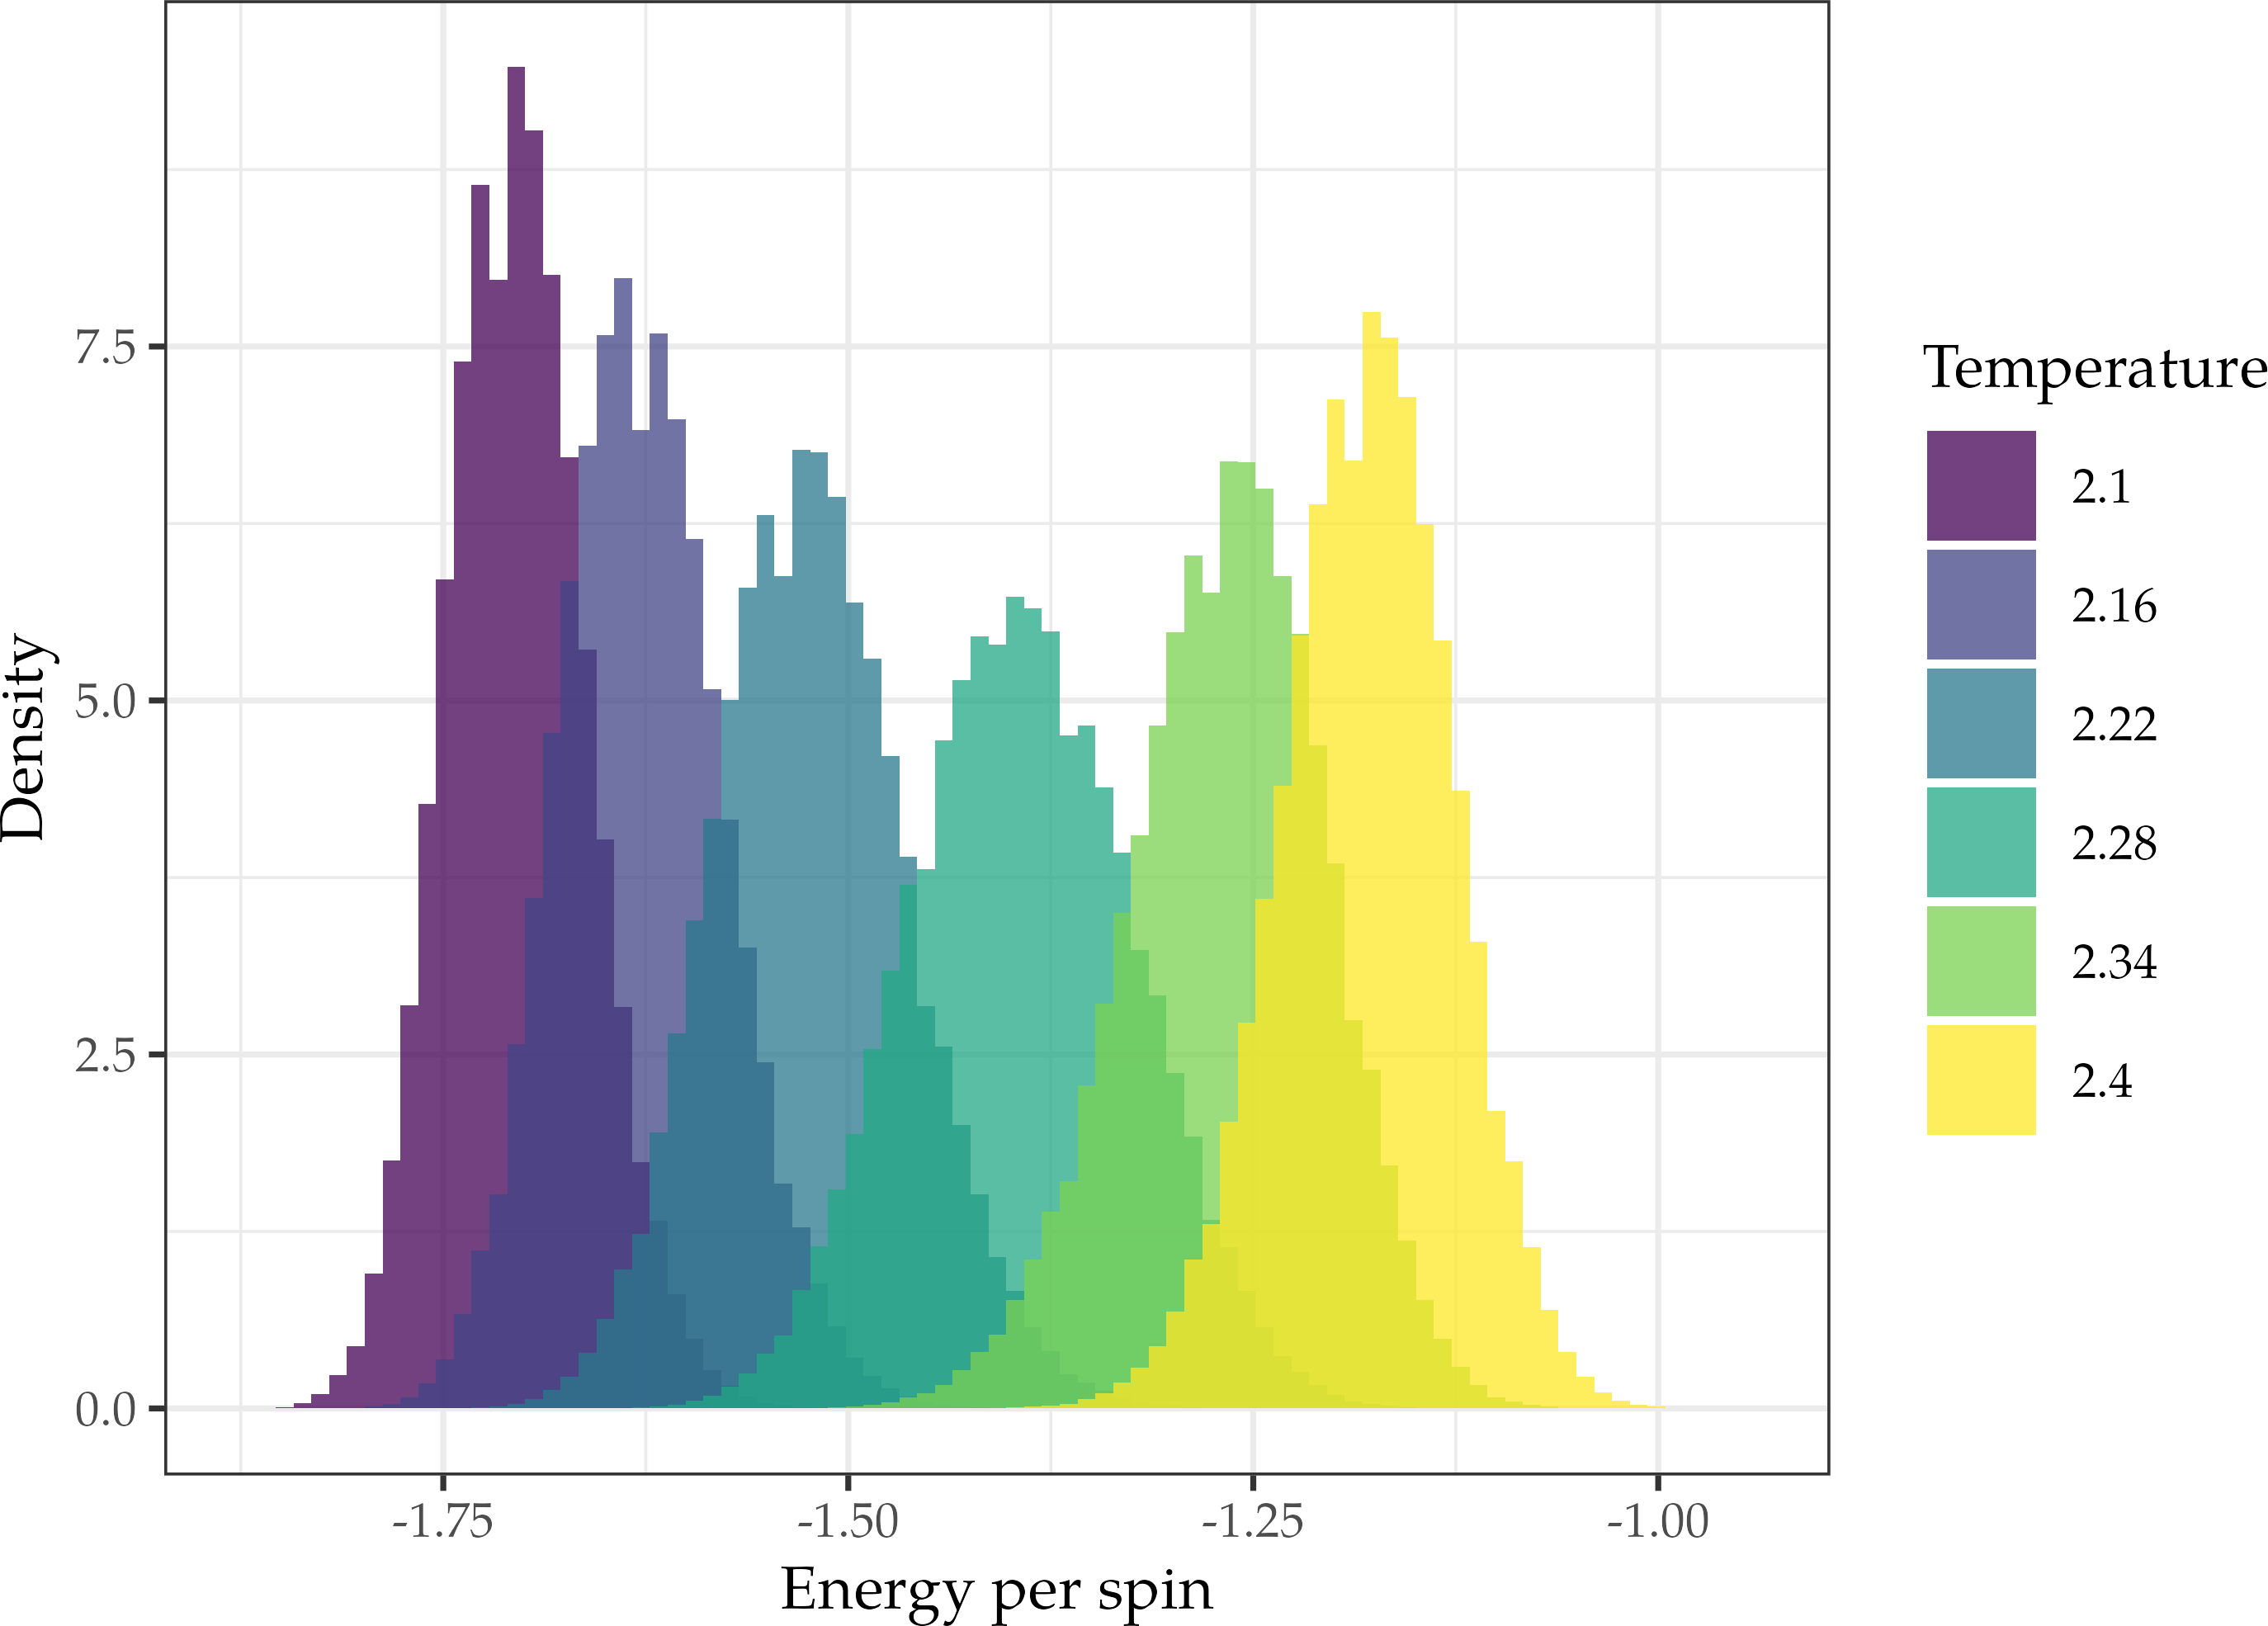
\includegraphics{img/062a}
  \caption{energy histograms for a \abbr{mmc} run with six chains, lattice size
    $L = 50$, \num{1000000} time steps with the first \num{1000} discarded for
    equilibration, and \num{20} steps between swap trials.}
  \label{fig:062a}
\end{figure}

\begin{table}
  \centering
  \captionabove{swapping rates -- i.e., the proportion of successful swaps --
    between the different chains for the \abbr{mmc} run referenced in
    \cref{fig:062a}. Each chain is identified by its respective temperature.}
  \label{tab:062a}
  \begin{tabular}{@{} c S[table-format=2.1] @{}}
    \toprule
    Chain temperatures & {Swapping rate (\%)} \\
    \midrule
    $\num{2.10} \leftrightarrow \num{2.16}$ & 26.6 \\
    $\num{2.16} \leftrightarrow \num{2.22}$ & 20.0 \\
    $\num{2.22} \leftrightarrow \num{2.28}$ & 16.5 \\
    $\num{2.28} \leftrightarrow \num{2.34}$ & 18.0 \\
    $\num{2.34} \leftrightarrow \num{2.40}$ & 28.5 \\
    \bottomrule
  \end{tabular} 
\end{table}

For the exercise, I performed a simulation with six chains at equispaced
temperatures between \num{2.1} and \num{2.4} and lattice size $L = \num{50}$.
This choice of temperatures leads to a good overlap in the energy distributions, as
seen in \cref{fig:062a}. Consequently, the swapping rates between the chains are
close to the recommended value of \qty{20}{\percent}, on average: the detailed
rates are reported in \cref{tab:062a}. The average over all chains is
\qty{22.8}{\percent}.

\begin{figure}
  \centering
  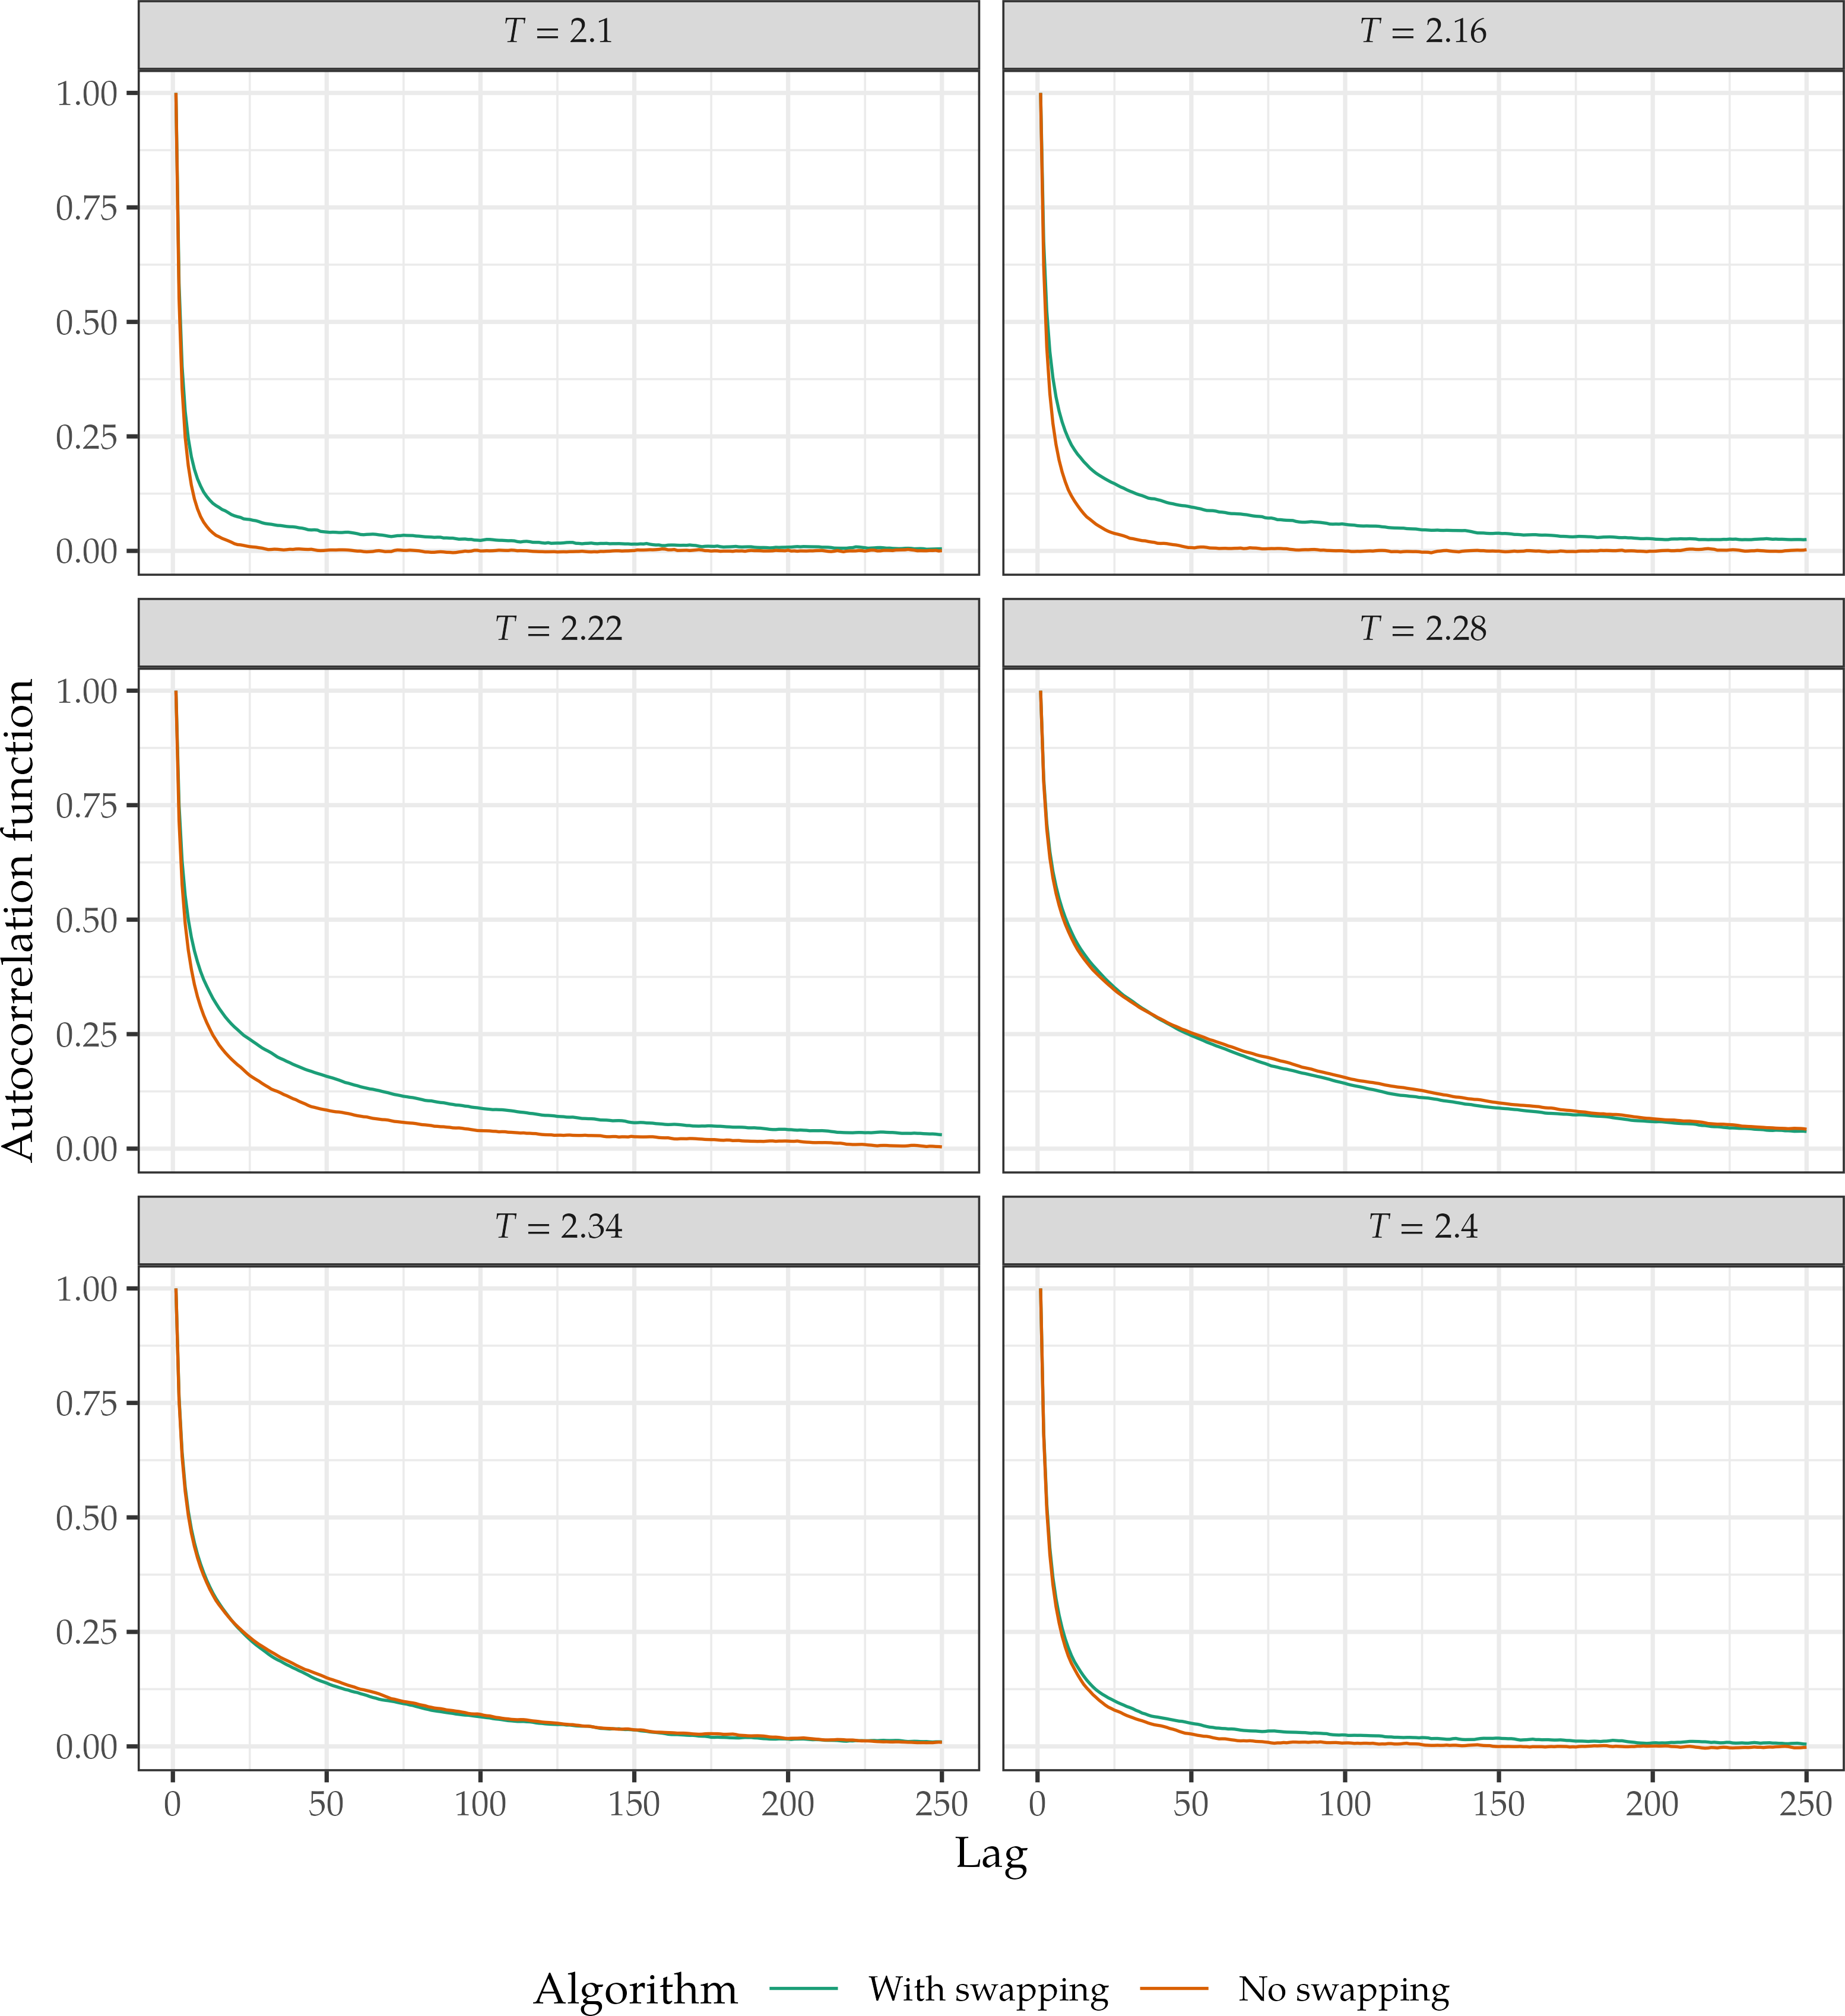
\includegraphics{img/062b}
  \caption{autocorrelation functions of the energy observations from the
    \abbr{mmc} simulations, with and without chain swapping.}
  \label{fig:062b}
\end{figure}

\begin{table}
  \centering
  \captionabove{autocorrelation times of the energy observations from the
    \abbr{mmc} simulations, with and without chain swapping.}
  \label{tab:062b}
  \begin{tabular}{
      @{} S[table-format=1.2] S[table-format=2.1] S[table-format=2.1]
  }
    \toprule 
    {Temperature} & {$\tau$ with swapping} & {$\tau$ without swapping} \\
    \midrule
    2.10 & 8.3 & 2.2 \\
    2.16 & 18 & 4.2 \\
    2.22 & 27 & 16 \\
    2.28 & 40 & 41 \\
    2.34 & 22 & 23 \\
    2.40 & 11 & 6.9 \\
    \bottomrule
  \end{tabular}
\end{table}

Next, I ran a new simulation with the same parameters but without allowing
swaps. In practice, this amounts to running six independent standard Metropolis
simulations at the chosen temperatures. I then compared the autocorrelation
times in the energy time series between the two approaches. Unexpectedly, I
encountered an issue I could not identify. As shown in \cref{fig:062b,tab:062b},
the autocorrelation functions above $T_{\mathrm{c}}$ are nearly identical
between the \abbr{mmc} and the \enquote{no swapping} dataset. However, at lower
temperatures swapping actually leads to \emph{more} autocorrelation! This
behaviour persisted with different temperatures, lattice sizes, and time
intervals between swaps.
